\subsection{User Interfaces}

\subsubsection{Mobile client}

\begin{figure}
  \centering
  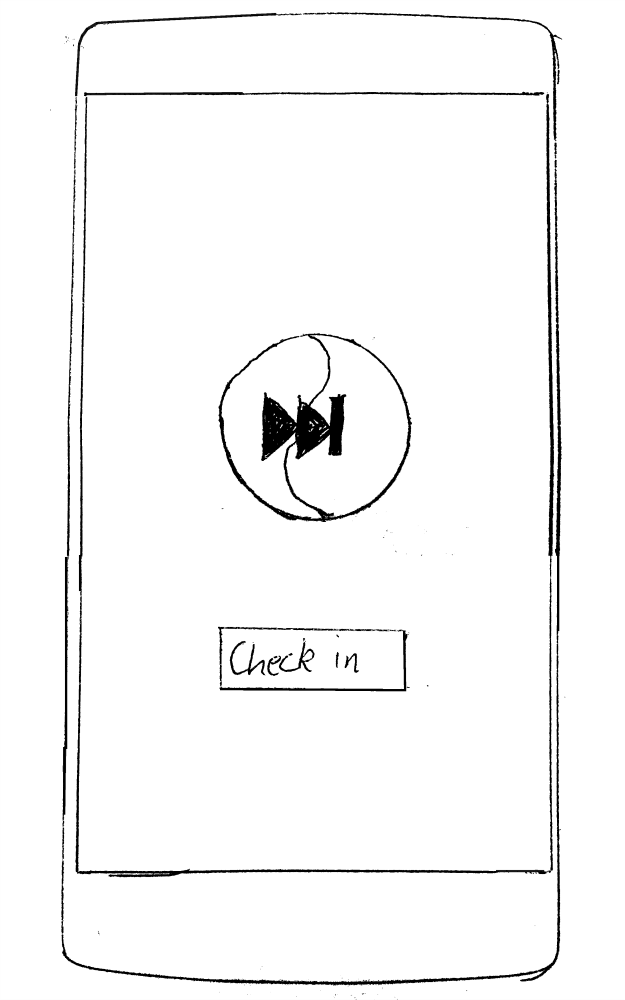
\includegraphics[width=0.25\linewidth]{Images/sketch1.png}
  \caption{Sketch1}
  \label{fig:sketch1}
\end{figure}

First the user is presented with the systems logo, and a single button. The caption of the button suggest to the user that, one is about to "check in". As shown in \cref{fig:sketch1}. When clicked user is presented a list of venues for the user to check in at, see \cref{fig:sketch2}.

\begin{figure}
  \centering
  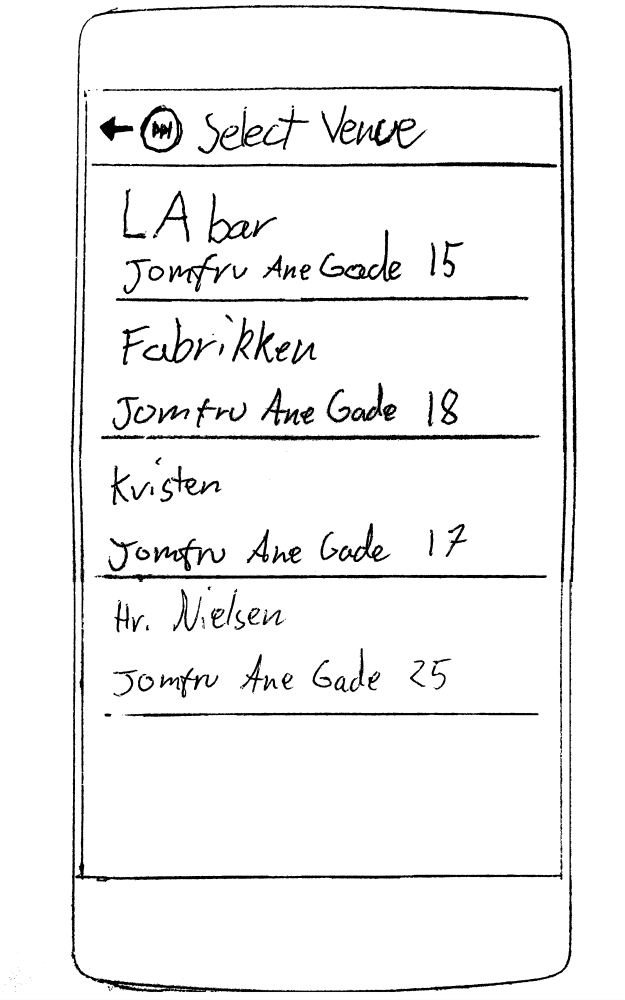
\includegraphics[width=0.25\linewidth]{Images/sketch2.png}
  \caption{Sketch2}
  \label{fig:sketch2}
\end{figure}

\begin{figure}
  \centering
  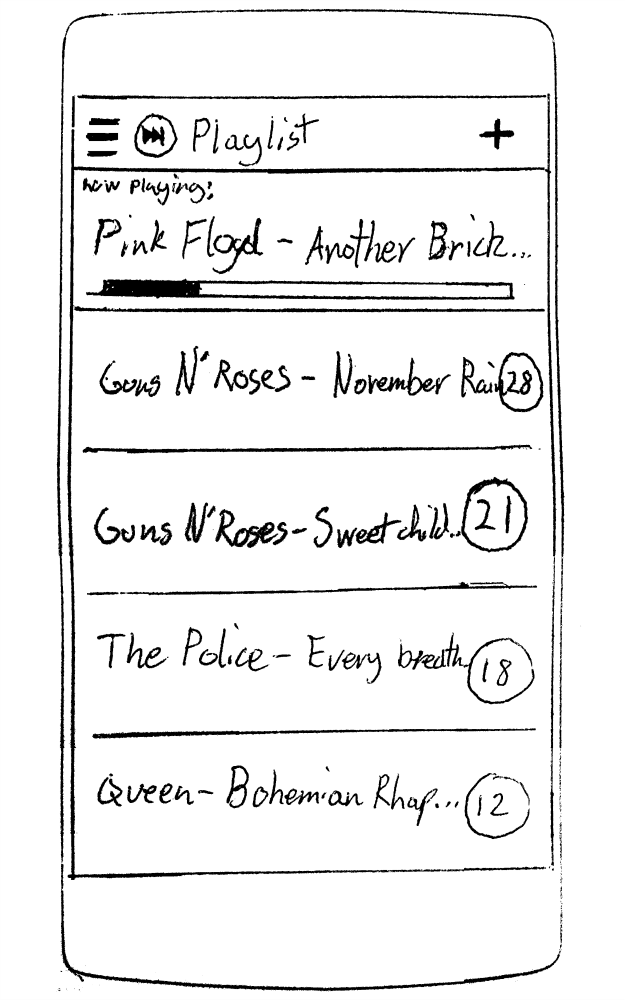
\includegraphics[width=0.25\linewidth]{Images/sketch3.png}
  \caption{Sketch3}
  \label{fig:sketch3}
\end{figure}

The user is now checked in at a venue and is presented with the playlist of the venue, including with is current playing. See \cref{fig:sketch3}. A little "+" icon suggest to perform an action of "addition", which in this context is adding to the playlist, if clicked the user can now browse through tracks and add them to the playlist. The "top" played tracks of that specific venue is display, or user can view publicly trending "hot" tracks. Shown in \cref{fig:sketch4}. Additionaly the magnifying glass at the very top is symbolising an action of searching, when clicked the user can search for specific tracks.

\begin{figure}
  \centering
  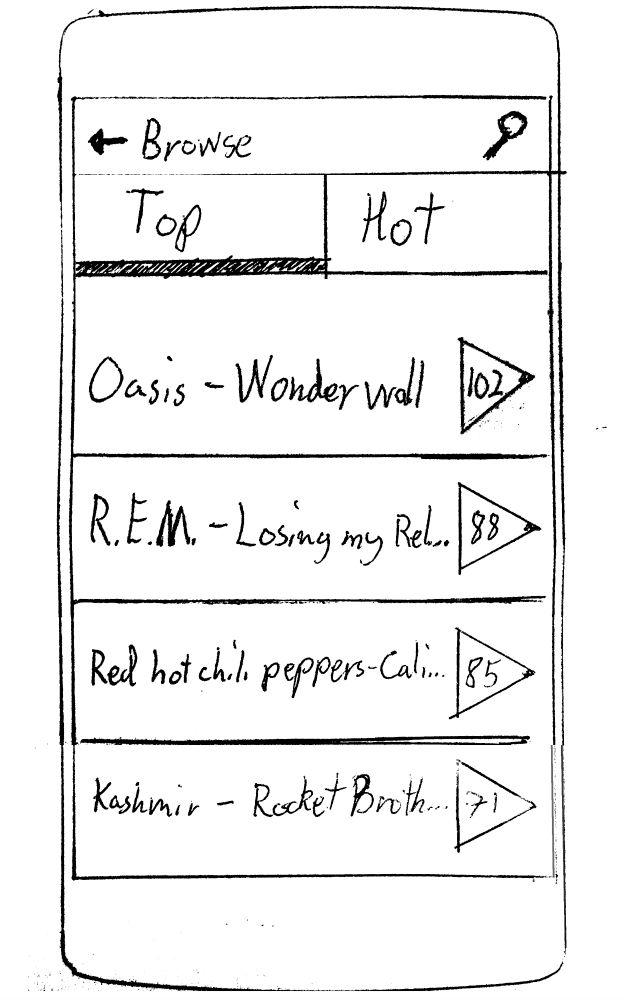
\includegraphics[width=0.25\linewidth]{Images/sketch4.png}
  \caption{Sketch4}
  \label{fig:sketch4}
\end{figure}
